\section*{Описание экспериментальной установки}

Схема экспериментальной установки для исследования дифракции Френеля на щели приведена на рисунке:

\begin{figure}[H]
	\centering
	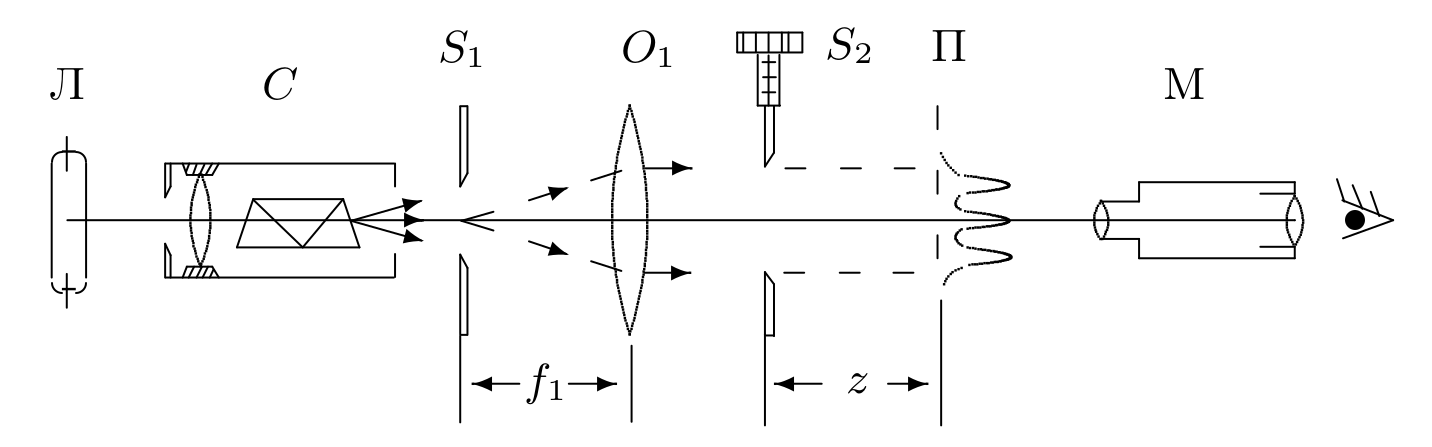
\includegraphics[width=0.9\textwidth]{../Изображения/Схема установки. Дифракция Френеля.png}
	\caption{Схема экспериментальной установки}
\end{figure}

Схема экспериментальной установки для исследования дифракции Фраунгофера на щели приведена на рисунке:

\begin{figure}[H]
	\centering
	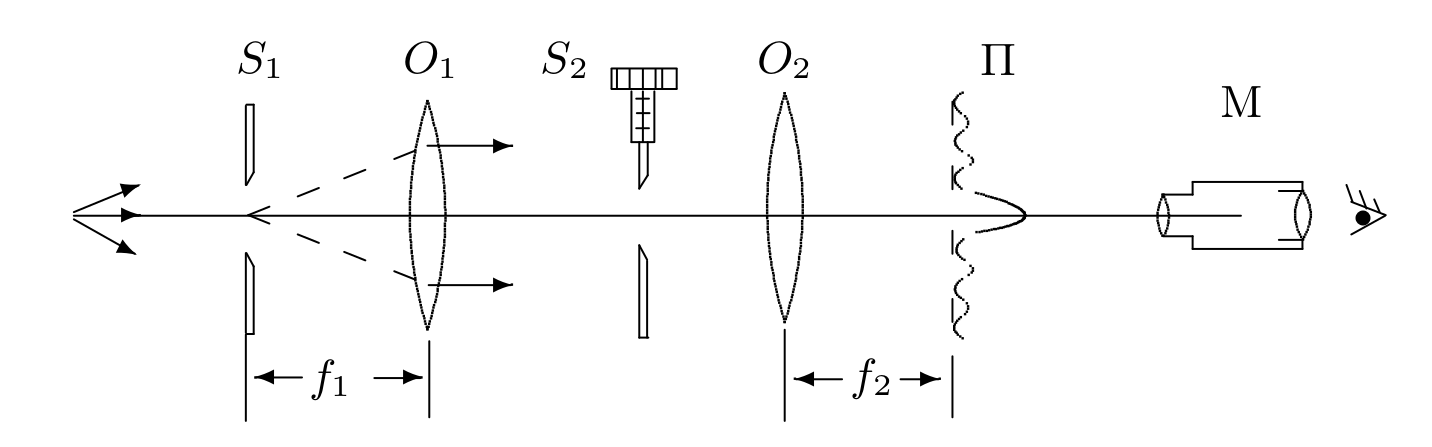
\includegraphics[width=0.9\textwidth]{../Изображения/Схема установки. Дифракция Фраунгофера.png}
	\caption{Схема экспериментальной установки}
\end{figure}

Схема экспериментальной установки для исследования дифракции Фраунгофера на двух щелях приведена на рисунке:

\begin{figure}[H]
	\centering
	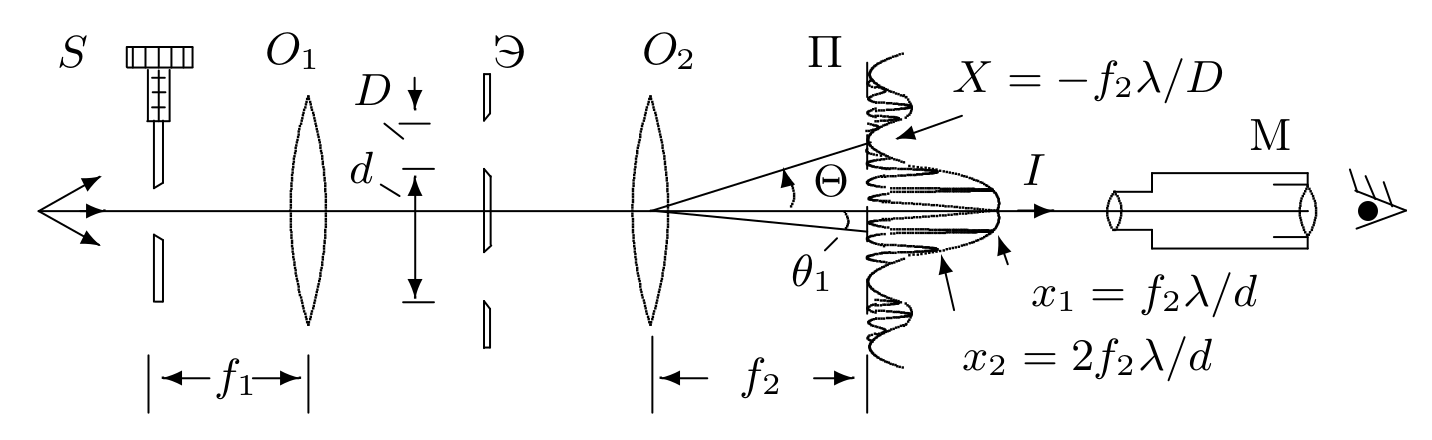
\includegraphics[width=0.9\textwidth]{../Изображения/Схема установки. Дифракция Фраунгофера, две щели.png}
	\caption{Схема экспериментальной установки}
\end{figure}


Схема экспериментальной установки для исследования влияния дифракции на разрешающую способность оптического прибора приведена на рисунке:

\begin{figure}[H]
	\centering
	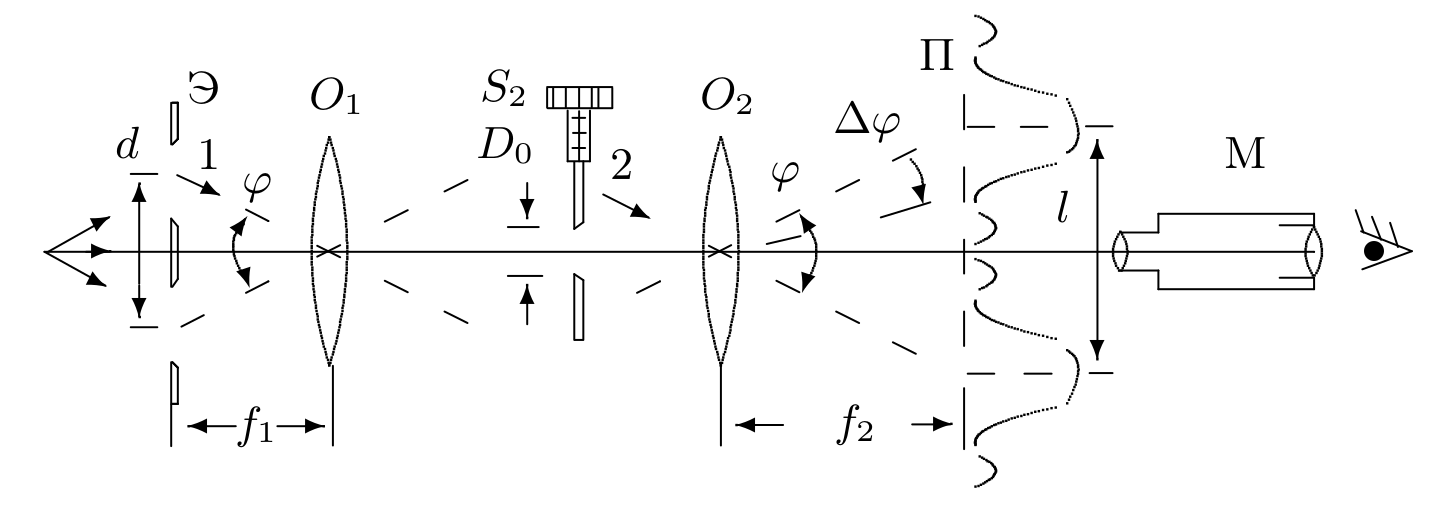
\includegraphics[width=0.9\textwidth]{../Изображения/Схема установки. Разрешающая способность.png}
	\caption{Схема экспериментальной установки}
\end{figure}

